\section{Capsule Network}
CNNs classify objects based on features they find in the image. When it spots a head, arms, legs and a body, it will classify the image as a person. However, spatial relationship between the features or their rotation is not considered. 

CapsNet \cite{capsnet2017} was developed to address this problem. A new neuron organisation called \textit{capsule} is proposed. Capsules are groups of neurons within one layer. Capsules output vectors (not scalars!), because they can encode more information. The size of the vector indicates the probability of the feature to even exist and its orientation describes various properties, like size, rotation, position, texture, etc. 

The proposed architecture (Fig \ref{fig:capsnet}) is quite simple. The first layer is convolutional and extracts features for capsules. The second layer is Primary Capsule layer. Consists of 32 capsules of 8 kernels and outputs 8D vectors. Those go to Digit Capsule Layer. This layer consists of 10 capsules (one capsule per class, in this case digits). All the capsules from the lower (primary) layer send their output to all the capsules in the higher (digit) level. The higher level outputs 16D vectors, which are fed to 3 fully connected layers. 

Dynamic routing is a process between two capsule layers. Its job is to replace max-pooling, during which spatial information is lost. Thanks to dynamic routing, output of one capsule gets send to the most appropriate parent capsule in the higher level. 

\begin{figure}[ht!]
    \centering
    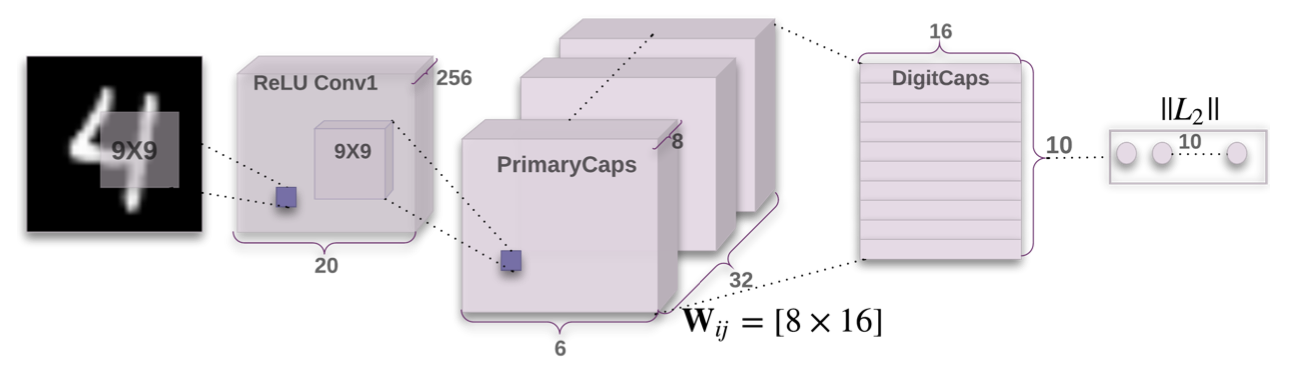
\includegraphics[width=300pt]{images/capsnet.png}
    \caption[CapsuleNetwork architecture]{CapsuleNetwork architecture \cite{capsnet2017}}
    \label{fig:capsnet}
\end{figure}

The model achieves very good results on classifying digits from MNIST and can also recognise overlapped digits in the MultiMNIST dataset. The way Capsule Networks work resembles human brain more than conventional CNNs. Even though they proved themselves successful on simple tasks like digit recognition, CapsuleNetworks are still a subject of research and need to improve their performance on more complex tasks. 